%
%  untitled
%
%  Created by Johan Boissard [] on 2010-06-24.
%  Copyright (c) Johan Boissard. All rights reserved.
% hhh

\documentclass[a4paper,titlepage] {scrartcl}
\usepackage[T1]{fontenc}
\usepackage[utf8]{inputenc}
\usepackage{graphicx}
\usepackage{engord}
%\usepackage[english]{babel}
\usepackage{fancyhdr}
\usepackage{amsmath}
\usepackage{comment}

\usepackage{listings}

%allows inclusion of url (hyperref is better than url) 
%ref: http://www.fauskes.net/nb/latextips/
\usepackage{hyperref}

%package for chemistry ie: \ce{(NH4)2SO4 -> NH4+ + 2SO4^2-} 
%ref:www.ctan.org/tex-archive/macros/latex/contrib/mhchem/mhchem.pdf
\usepackage[version=3]{mhchem}
%celsius + degrees
\usepackage{gensymb}
%to get last page
\usepackage{lastpage} % \pageref{LastPage}

%make use of the fullpage (no HUGE margins)
\usepackage{fullpage}
\usepackage{subfig}

%allows separating cell in table by diagonal line
\usepackage{slashbox}




%\renewcommand{\chaptername}{Laboratory}
%\setcounter{chapter}{5}

\usepackage{color}
\usepackage[usenames,dvipsnames, table]{xcolor}
% Include this somewhere in your document



\usepackage[absolute]{textpos}

%column  of multi row in tables
\usepackage{multirow}

%to have vertical text in table
\usepackage{rotating}


%%%%%%% a virer ici!!!!
\begin{comment}
%Fonts and Tweaks for XeLaTeX
\usepackage{fontspec,xltxtra,xunicode}
%\defaultfontfeatures{Mapping=tex-text}
%\setromanfont[Mapping=tex-text]{Hoefler Text}
\setsansfont[Scale=MatchLowercase,Mapping=tex-text]{Gill Sans}

\definecolor{shade}{HTML}{D4D7FE}	%light blue shade
\definecolor{text1}{HTML}{272727}		%text is almost black
\definecolor{headings}{HTML}{173849} 	%dark blue %%%dark red 70111
\definecolor{title}{HTML}{173849} 	%dark blue %%%dark red 70111

\usepackage{titlesec}				%custom \section
\end{comment}







\author{Johan Boissard}
\date{\today}
\title{Marketing}
\begin {document}


\maketitle
\tableofcontents
\newpage

\begin{comment}
	
\section{Process général}
\begin{enumerate}
	\item Projet créé (sur project.studiocraft.ch)
	\item Appel d'offre
	\item Création du design
	\item Validation du design
	\item Mise en place du CMS
	\item Mise en place du contenu
	\item Installation sur serveur
	\item Enquête de satisfaction \footnote{Idéalement se fait directement lors du passage à "fin de mandat"}
	\item Fin du mandat
\end{enumerate}

\section{Process compta} % (fold)
\begin{enumerate}
	\item Demande de facture (par collabo)
	\item Facture envoyée
	\item Facture payée
\end{enumerate}
\label{sec:process_compta}

% section process_compta (end)
\end{comment}
\section{Intro}	

Value is perceived measure
\begin{equation}
	\text{Value}_{\text{perceived}} = \frac{\text{benefit}_{\text{perceived}}}{\text{cost}_{\text{perceived}}}
\end{equation} 
Perceived value
\begin{itemize}
	\item Delivery on time
	\item Technological performance
	\item Information about product
	\item Soft performance
\end{itemize}

\section{Marketing Strategy}

\begin{enumerate}
	\item Marketing strategy
	\begin{enumerate}
		\item Market \textbf{Segmentation}
		\item Market \textbf{Targeting}
		\item Market \textbf{Positioning}
	\end{enumerate}
\end{enumerate}


\subsection{Segmentation} % (fold)
divide up the market into segments

Segment: subgroup of people sharing characteristics cause similar needs

Segmentation: dividing the market for customer needs 

\paragraph{Requirements for successful segmentation} % (fold)
\begin{itemize}
	\item \textbf{Identifiable} segments are empirically detectable
	\item \textbf{Accessible} segments are reachable through communication and distribution channells
	\item \textbf{Durable} segments msut be realtively stable to minimize the cost of frequent changes
	\item \textbf{Substantial} segments are large enough to be profitable
	\item \textbf{Unique} segments must respond to different stimuli
\end{itemize}



% paragraph  (end)

\paragraph{Segmentation variables for consumer markets} % (fold)
\label{par:segmentation_variables_for_consumer_markets}

\begin{itemize}
	\item Geographic
	\item Demographic
	\item Psychographic
	\item Behavioral
\end{itemize}


\paragraph{Segmentation process} % (fold)
\label{par:segmentation_process}
\begin{enumerate}
	\item Identify customer value
	\item Segment the market
	\item Find proxies
\end{enumerate}


% paragraph segmentation_process (end)
% paragraph segmentation_variables_for_consumer_markets (end)

\subsection{Targeting}

A set of buyers share common needs that you decide to serve

\paragraph{Rationale behind targeting} % (fold)
\label{par:rationale_behind_targeting}
\begin{itemize}
	\item External
	\begin{itemize}
		\item Segment size
		\item segment growth
		\item segment attractiveness
	\end{itemize}
	\item Internal
	\begin{itemize}
		\item company objectives
		\item company resources
	\end{itemize}
\end{itemize}

outcome can be
\begin{itemize}
	\item Differentiated
	\item Undifferentiated
	\item Concentrated
\end{itemize}



% paragraph rationale_behind_targeting (end)


\paragraph{Key questions} % (fold)
\label{par:key_questions}
\begin{itemize}
	\item perceived value better than in other segments?
	\item how can segment be reached?
	\item how quick?
	\item how big is segment?
\end{itemize}
% paragraph key_questions (end)

\subsection{Positioning}
\begin{itemize}
	\item Why me rather than competitor?
	\item unique differentiated features as perceived by segment?
\end{itemize}

Positioning forms the basis for the marketing mix
\begin{figure}[htbp]
	\centering
		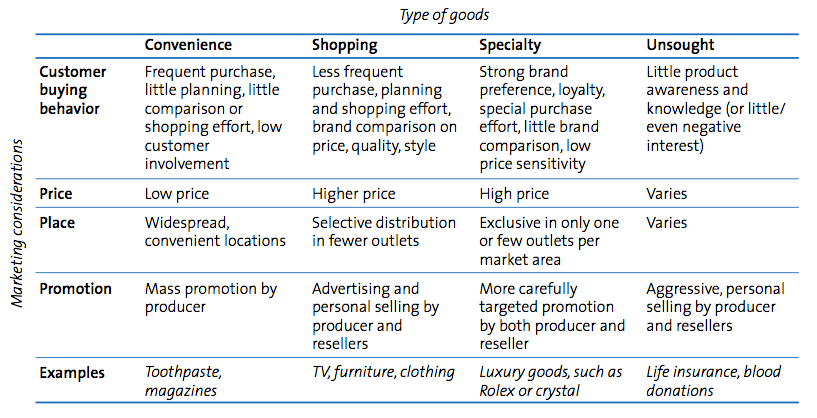
\includegraphics[height=3in]{images/position.png}
	\caption{Generic positioning}
	\label{fig:images_position}
\end{figure}

\section{Product} % (fold)
\label{sub:product}
A product can be defined as anything that is offered to the market for consumption...
and that satisfies a \emph{need}.

Two categories of goods
\begin{itemize}
	\item \textbf{tangible}: physical products
	\item \textbf{intangible}: services, events, people, places, ideas, ...
\end{itemize}

Can also be classified as
\begin{itemize}
	\item \textbf{Nature of customer's buying behavior} convenience goods, shopping goods, or specialty goods
	\item \textbf{Level of involvement in purchase process} low (customer), high (industrial)
	\item \textbf{Type of customer benefit} functional or emotional
\end{itemize}

\paragraph{Product Line} % (fold)
\label{par:product_line}
is a group of items satisfying \textbf{similar} customer \textbf{needs}

A \textbf{Product mix} encompasses \textbf{all product lines}

A product line has two dimensions
\begin{itemize}
	\item \textbf{depth} number of versions of each product in the line
	\item \textbf{length} number of products within a product line
\end{itemize}
% paragraph product_line (end)

\paragraph{Product augmentation} % (fold)
\label{par:product_augmentation}
\begin{figure}[htbp]
	\centering
		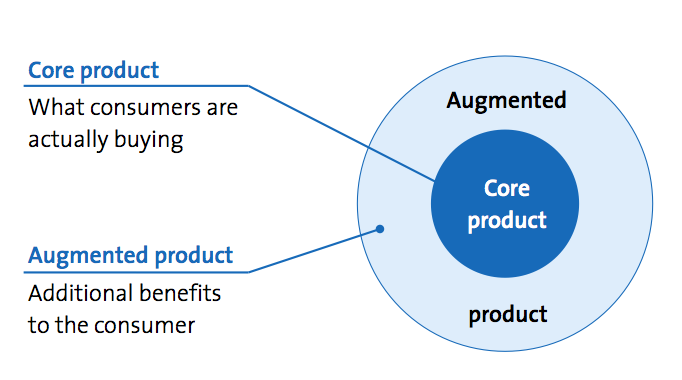
\includegraphics[height=2.5in]{images/morethanproduct.png}
	\caption{There is more than the product itself}
	\label{fig:images_morethanproduct}
\end{figure}

The augmented product provides additional benefits
examples
\begin{itemize}
	\item customer service
	\item installation
	\item repair and delivery service
	\item warranty
	\item credit possibilities
\end{itemize}

% paragraph product_augmentation (end)

\paragraph{Brand} % (fold)
\label{par:brand}
Names and symbols that make \textbf{product differentiation} concrete. Identity, quality, consistency, legal protection , segmentation.
\begin{figure}[htbp]
	\centering
		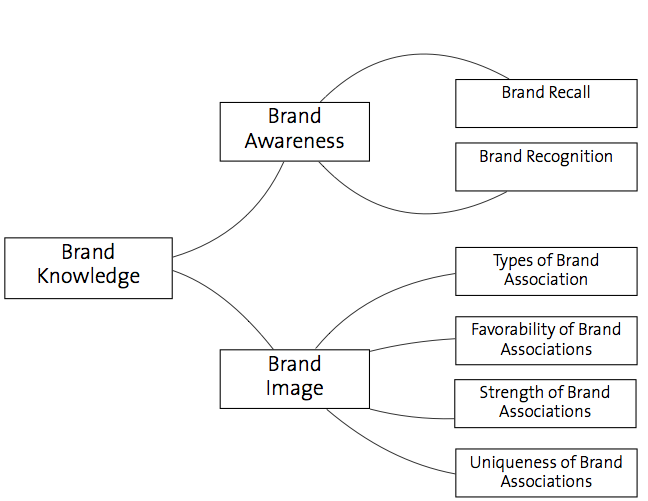
\includegraphics[height=3in]{images/brand.png}
	\caption{Brand}
	\label{fig:images_brand}
\end{figure}

Brand awareness: can you \textbf{identify} the brand?\\
Brand image: what do you identify the brand with ?

Brand can be augmented.
% paragraph brand (end)

% subsection product (end)

\section{Place} % (fold)
\label{sub:product}

\subsection{Marketing Channel}
Marketing channels connect to customers

\begin{itemize}
	\item The set of mechanisms or the network via the the firm goes to market
	\item How the seller \textbf{places the product} in the hands of the buyer
	\item Selling, transporting, storing, and \textbf{making goods available} for the customer
	\item Marketing channels are sets of \textbf{interdependent organizations} that help make a product or servic available for consumption
\end{itemize}

Marketing channels have four main functions
\begin{itemize}
	\item \textbf{Demand generation} - sales generation - how the customer acquires the product
	\begin{itemize}
		\item Direct vs indirect
		\begin{itemize}
			\item mom and pop store
			\item internet store
			\item warehouse store
		\end{itemize}
		\item differences to consider
		\begin{itemize}
			\item interaction
			\item availability
			\item price
		\end{itemize}
	\end{itemize}
	
	\item \textbf{Demand fulfillment} - distribution channel - how the product reaches the customer
	\begin{itemize}
		\item direct vs indirect
		\item distribution channels provide products where and when customers want them
	\end{itemize}
	\item After-sale service	
	\item Information/ market feedback for strategy development
\end{itemize}



\paragraph{Consumer and business channels} % (fold)
\label{par:consumer_and_business_channels}
can be of different lengths. Different terminology for business or private customer.
\begin{itemize}
	\item \textbf{Private}: $\rightarrow$
	 						(wholesaler) 
							$\rightarrow$ 
							retailer
	\item \textbf{Business}: $\rightarrow$ (manufacturer's representative of sales branch) $\rightarrow$ business distributor
\end{itemize}

% paragraph consumer_and_business_channels (end)


\subsection{Intermediaries}
Much less connections with an intermediary. ($3\cdot3=9$ vs $3+3=6$)

\begin{itemize}
	\item Increase reach of products
	\item Lower cost of sales and distribution
	\item Facilitate search by customers
\end{itemize}
 
Can be a company sales force, manufacturer's agency, industrial distributors, wholesaler, retailer, ...

Intermediaries \textbf{bridge} place and possession \textbf{gaps} that separate goods and services from those that would use them.

Payment intermediaries facilitate financial transactions between buyers and sellers. Payment intermediaries \textbf{bridge } the trust gaps that separate buyers and sellers.




\subsection{Direct vs indirect channel}

\begin{itemize}
	\item Direct sales: no independent party exists between firm and customer for selling
	\item indirect sales: independent party for selling
	\item Direct distribution: no independent party exists between firm and customer to distribute the product
	\item Indirect distribution: independent party exists for distributing product.
\end{itemize}
\underline{Examples:}\\
direct + direct: IKEA (warehouse), Nike (brands)\\
direct distribution + indirect sale: sales represent or through specialized agencies (airlines, hotels)\\
indirect + indirect: retail stores, wholesalers or business distributors\\
direct sale but indirect distribution: no change in ownership -> outsourced distribution

From the perspective of a manufacturer, retailing companies enable indirect sales and distribution:\\
\textbf{retailing}: all activities involved in selling goods or services directly to final customers for their \textbf{personal, nonbusiness use}
\\
\textbf{wholesaling}: all-activities involved in selling goods and services to those buying for resale of \textbf{business} use.


\paragraph{Various types of direct sales} % (fold)
\label{par:various_types_of_direct_sales}
Personal | non-personal and physical | non-physical
% paragraph various_types_of_direct_sales (end)
% subsection product (end)

\subsection{Channel decisions} % (fold)
\label{sub:channel_decisions}
Factors influencing channel decisions
\begin{itemize}
	\item sales cycle
	\item nature of the selling task
	\item personal relations
	\item product line
	\item target market
	\item customer location
	\item product development
	\item order size
	\item order placement
	\item after-sales service
\end{itemize}


The channel breadth is the number of distribution points in each layer.
\begin{itemize}
	\item Convenience good
	\item Specialty good
	\item Shopping good
\end{itemize}


\paragraph{A framework for designing marketing channels} % (fold)
\label{par:a_framework_for_designing_marketing_channels}
\begin{enumerate}
	\item Identify homogeneous segments
	\item Identifying customer's channel function requirements
	\item Benchmarking own and competitors' capabilities with requirements
	\item Develop options that satisfy customers' requirements
	\item Evaluate options
	\item Analyze channel overlaps
\end{enumerate}

Several conflict can occur
\begin{itemize}
	\item Horizontal conflict: between two channels
	\item Vertical: within channel
	\item Dual distribution conflict: business vs personal
\end{itemize}
% paragraph a_framework_for_designing_marketing_channels (end)

% subsection channel_decisions (end)


\section{Promotion} % (fold)
\label{sec:promotion}
The paid activities or events that provide inducements to customers to do something
\begin{itemize}
	\item Get people to hear about the company
	\item Get product in front of customers, channel intermediaries or press
	\item Provide temporary inducement for buying or trying product
\end{itemize}

\subsection{Promotion Mix} % (fold)
\label{sub:promotion_mix}
\subsubsection{Advertising}	 % (fold)
\label{par:advertising}
Any paid form of non-personal presentations and promotion of ideas, goods or services by an identified sponsor using one-way communication with a controlled message.

There are several types of advertising
\begin{itemize}
	\item Informative advertising
	\item Persuasive advertising
	\item Reminder advertising
\end{itemize}
% paragraph advertising (end)

\subsubsection{Sales promotion} % (fold)
\label{par:sales_promotion}
Non-personal short term incentives to encourage the immediate purchase or sale, usage or trial of a product or service

\underline{Examples:}
\begin{itemize}
	\item Coupons
	\item Discounts
	\item Contests
	\item Point of purchase display
	\item Rebates
	\item Gifts
	\item Free sampless
\end{itemize}
% paragraph sales_promotion (end)

\subsubsection{Public relations} % (fold)
\label{par:public_relations}
Building good relations with the company's various publics by obtaining favorable publicity, developing a good "corporate image", and handling or heading off unfavorable rumors, stories and events.
% paragraph public_relations (end)
% subsection promotion_mix (end)

\subsubsection{Personal selling}
Personal two-way presentation  by the firm's sales force for the purpose of making sales and building customer relationships.

\subsubsection{Direct Marketing}
\begin{itemize}
	\item Direct connections (without intervening media) with carefully targeted individuals customers to both obtain an immediate response and cultivating lasting customer relationships
	\item Focused on driving purchases attributed to a specific "call to action", thus effectiveness measured directly
	\item Direct mail, telemarketing, email, etc...
\end{itemize}

\subsubsection{Other forms}
\begin{itemize}
	\item What if others can help communicating our message ?
	\item Viral marketing
	\item  Giving it away for free can yield everlasting returns
	\item Loyalty programs communicate a sense of belonging
	\item Creativity is border less - but make sure to get it right ! (Tele2 case)
\end{itemize}


\subsection{Communication Process}
In order to get the customer to purchase, the buyer-readiness has to be developed through stages.
\begin{equation}
	\text{Awareness}\rightarrow
	\text{Knowledge}\rightarrow
	\text{Liking}\rightarrow
	\text{Preference}\rightarrow
	\text{Conviction}\rightarrow
	\text{Purchase}
\end{equation}

\paragraph{Steps in effective marketing communication} % (fold)
\label{par:steps_in_effective_marketing_communication}
Marketing communication needs to be structured along five steps

\begin{itemize}
	\item Identify target audience and characteristics
	\item Determine communication objectives
	\item Construct message
	\item Select media
	\item Collect feedback
\end{itemize}
% paragraph steps_in_effective_marketing_communication (end)

\paragraph{AIDA} % (fold)
\label{par:aida}
\begin{itemize}
	\item get \textbf{A}ttention
	\item Hold \textbf{I}nterest
	\item Arouse \textbf{D}esire
	\item Obtain \textbf{A}ction
\end{itemize}
% paragraph aida (end)


\paragraph{Constructing a message - select media} % (fold)
\label{par:constructing_a_message_select_media}
\begin{itemize}
	\item \textbf{Personal communication channels}
	\begin{itemize}
		\item Word of mouth
		\item Important when products are expensive, dangerous or highly visible
	\end{itemize}
	\item \textbf{Non-personal communication channel}
	\begin{itemize}
		\item Major media
		\item Atmospheres
		\item Events
	\end{itemize}
\end{itemize}
% paragraph constructing_a_message_select_media (end)

\subsection{Changes in marketing communication model}	
\begin{itemize}
	\item less \textbf{broadcasting} more \textbf{narrowcasting}
	\item Decline in television, magazines, and other mass media
	\item Emergence of highly fragmented needs and market
	\item Specialized, highly targeted media to reach smaller customer segments with personalized messages
	\item New channels building on new technologies
\end{itemize}

\paragraph{New communication channels} % (fold)
\label{par:new_communication_channels}
\begin{itemize}
	\item One-to-one marketing (web shop)
	\item Personalized media (RSS, podcasts)
	\item The long tail 
	\item Geo-marketing
\end{itemize}
% paragraph new_communication_channels (end)

\begin{equation}
	\Rightarrow
	\text{Challenge is to "cut through the clutter" and get noticed}
\end{equation}

% section promotion (end)

\section{Price}

\subsection{What is price ?} % (fold)
\label{sub:what_is_price_}
\begin{itemize}
	\item Sum of values that customers give up in order to gain the benefits of having or using a product or service
	\item amount of money charged for a product or service
	\item price is one of the most flexible marketing mix instrument
	\item price is the only instrument in the marketing mix that produces revenues; all other elements represent costs.
	
\end{itemize}
% subsection what_is_price_ (end)


\subsection{Cost - vs. value based pricing}
\begin{itemize}
	\item \textbf{Cost-based pricing}
			\begin{equation}
				\text{Product}\Rightarrow
				\text{Cost}\Rightarrow
				\text{Price}\Rightarrow
				\text{Value}\Rightarrow
				\text{Customers}
			\end{equation}
	\item \textbf{Value-based pricing}
			\begin{equation}
				\text{Customers}\Rightarrow
				\text{Value}\Rightarrow
				\text{Price}\Rightarrow
				\text{Cost}\Rightarrow
				\text{Product}
			\end{equation}
\end{itemize}

\paragraph{Cost based pricing (markup)} % (fold)
\label{par:cost_based_pricing_markup_}
\begin{equation}
	\text{Unit cost} = \text{Variable cost} + \frac{\text{Fixed costs}}{\text{Unit sales}}
\end{equation}

\begin{equation}
	\text{Markup price} = \frac{\text{Unit cost}}{1-\text{Desired return on sales}}
\end{equation}
% paragraph cost_based_pricing_markup_ (end)

Price can also be derived based on target profits at given cumulative quantities.

For each price there is (normally) a break-even volume, at which the sales turns profitable.

\subsection{Pricing strategies}
\begin{tabular}{ccccc}
\hline
 & Competitive & Monopolistic& Oligopoly & Monopoly\\
\hline
Charactiersitics\\of market\\environments & trading uniform commodities\\& differentiated goods & few sellers & one seller\\
\hline
Seller's degree of freedom & price taker & price range & sensitive to other's prices & free or regulated price\\
\hline
\end{tabular}

The more elastic the demand, the stronger it reacts to a change in price

\paragraph{Throuhout the liecycle of a product, different pricing strategies come in place} % (fold)
\label{par:throuhout_the_liecycle_of_a_product_different_pricing_strategies_come_in_place}
\begin{itemize}
	\item Introduction
	\begin{itemize}
		\item Market skimming pricing
		\item Market penetration pricing
	\end{itemize}
	\item Maturity
	\begin{itemize}
		\item Product line pricing
		\item Captive product pricing
		\item Product bundle pricing
	\end{itemize}
	\item Decline
	\begin{itemize}
		\item Price adjustment strategies
	\end{itemize}
\end{itemize}
% paragraph throuhout_the_liecycle_of_a_product_different_pricing_strategies_come_in_place (end)

\subsubsection{Market skimming price}
\begin{itemize}
	\item Characteristics
	\begin{itemize}
		\item High initial price reduction
		\item Subsequent price reduction
		\item Skim segments willing to pay premium
	\end{itemize}
	\item Requirements
	\begin{itemize}
		\item Quality and image must support higher price
		\item Cost efficient production of small volumes
		\item entry barriers, competitors cannot undercut
	\end{itemize}
\end{itemize}

\subsubsection{Market penetration pricing}
\begin{itemize}
	\item Characteristics
	\begin{itemize}
		\item Low initial price for new product
		\item Attract many buyers fast, win market share
		\item Logic: High volumes $\rightarrow$ low costs
	\end{itemize}
	\item Requirements
	\begin{itemize}
		\item Price sensitive market (elastic demand)
		\item Production and distribution costs must fall with volume increase
		\item Low price keeps out competition (cost advantage)
	\end{itemize}
\end{itemize}

\subsubsection{Product line pricing}
\begin{itemize}
	\item Setting price differences between product line items
	\item Simplified pricing
	\item Cost differences
	\item Customer evaluation of different features
	\item Competitor prices
\end{itemize}

\subsubsection{Captive product pricing}
\begin{itemize}
	\item Setting prices for products that must be used along with a main product
	\item Low entry cost
	\begin{itemize}
		\item induce usage
		\item high captive product prices
		\item high usage cost
	\end{itemize}
	\item Services: two-part pricing
	\begin{itemize}
		\item fixed fees
		\item variable usage rate
	\end{itemize}
\end{itemize}

\subsubsection{Product bundle pricing}
\begin{itemize}
	\item Combining several products
	\item Offering bundle at reduced price
	\item Can promote the sales of products which consumers might not otherwise buy
	\item however, combined price must be low enough to get them to buy the bundle
\end{itemize}

\subsubsection{Price-adjustment strategies}
adjusting prices to account for customers differences and changing situations

\paragraph{Discount pricing} % (fold)
\label{par:discount_pricing}
A straight reduction in price on pruchases during a stated period of time
% paragraph discount_pricing (end)

\paragraph{Allowance pricing} % (fold)
\label{par:allowance_pricing}
bla bla bla
% paragraph allowance_pricing (end)

\paragraph{Segmented price} % (fold)
\label{par:segmented_price}
Selling the same product for two different prices. The segmented prices must reflect the differences in customers' perceived value
% paragraph segmented_price (end)

\paragraph{Psychological pricing} % (fold)
\label{par:psychological_pricing}
\begin{itemize}
	\item Pricing cues
	\item High price = high quality ?
	\item Reference price
	\item Sale signs
	\item Prices ending in 9
	\item Pricing matching guarantee
\end{itemize}
% paragraph psychological_pricing (end)

\paragraph{Promotional pricing} % (fold)
\label{par:promotional_pricing}
\begin{itemize}
	\item Temporarily pricing below the list price (or even cost)
	\item Increase short-run sales
	\item Can lead to price wars
	\item Easily copied
\end{itemize}

"Price promotions are the brand equivalent of heroine: easy to get into but hard to get out of"

and remember... "there is no such things as a free lunch"

% paragraph promotional_pricing (end)

\end{document}
